% Options for packages loaded elsewhere
\PassOptionsToPackage{unicode}{hyperref}
\PassOptionsToPackage{hyphens}{url}
%
\documentclass[
]{article}
\usepackage{lmodern}
\usepackage{amssymb,amsmath}
\usepackage{ifxetex,ifluatex}
\ifnum 0\ifxetex 1\fi\ifluatex 1\fi=0 % if pdftex
  \usepackage[T1]{fontenc}
  \usepackage[utf8]{inputenc}
  \usepackage{textcomp} % provide euro and other symbols
\else % if luatex or xetex
  \usepackage{unicode-math}
  \defaultfontfeatures{Scale=MatchLowercase}
  \defaultfontfeatures[\rmfamily]{Ligatures=TeX,Scale=1}
\fi
% Use upquote if available, for straight quotes in verbatim environments
\IfFileExists{upquote.sty}{\usepackage{upquote}}{}
\IfFileExists{microtype.sty}{% use microtype if available
  \usepackage[]{microtype}
  \UseMicrotypeSet[protrusion]{basicmath} % disable protrusion for tt fonts
}{}
\makeatletter
\@ifundefined{KOMAClassName}{% if non-KOMA class
  \IfFileExists{parskip.sty}{%
    \usepackage{parskip}
  }{% else
    \setlength{\parindent}{0pt}
    \setlength{\parskip}{6pt plus 2pt minus 1pt}}
}{% if KOMA class
  \KOMAoptions{parskip=half}}
\makeatother
\usepackage{xcolor}
\IfFileExists{xurl.sty}{\usepackage{xurl}}{} % add URL line breaks if available
\IfFileExists{bookmark.sty}{\usepackage{bookmark}}{\usepackage{hyperref}}
\hypersetup{
  hidelinks,
  pdfcreator={LaTeX via pandoc}}
\urlstyle{same} % disable monospaced font for URLs
\usepackage[margin=1in]{geometry}
\usepackage{graphicx,grffile}
\makeatletter
\def\maxwidth{\ifdim\Gin@nat@width>\linewidth\linewidth\else\Gin@nat@width\fi}
\def\maxheight{\ifdim\Gin@nat@height>\textheight\textheight\else\Gin@nat@height\fi}
\makeatother
% Scale images if necessary, so that they will not overflow the page
% margins by default, and it is still possible to overwrite the defaults
% using explicit options in \includegraphics[width, height, ...]{}
\setkeys{Gin}{width=\maxwidth,height=\maxheight,keepaspectratio}
% Set default figure placement to htbp
\makeatletter
\def\fps@figure{htbp}
\makeatother
\setlength{\emergencystretch}{3em} % prevent overfull lines
\providecommand{\tightlist}{%
  \setlength{\itemsep}{0pt}\setlength{\parskip}{0pt}}
\setcounter{secnumdepth}{-\maxdimen} % remove section numbering
\usepackage{setspace}\doublespacing
\usepackage{lineno}\linenumbers

\author{}
\date{\vspace{-2.5em}}

\begin{document}

\hypertarget{estimates-of-phylogenetic-signal-based-on-lambda-are-often-inaccurate}{%
\section{Estimates of Phylogenetic Signal Based on Lambda are Often
Inaccurate}\label{estimates-of-phylogenetic-signal-based-on-lambda-are-often-inaccurate}}

\hfill\break

\textbf{Keywords}: Pagel's lambda, phylogenetic signal \hfill\break

\textbf{Short Title}: Inaccuracies in Pagel's Lambda \hfill\break

\hypertarget{abstract}{%
\section{Abstract}\label{abstract}}

\{conclusion holds: interpreting the regression is not appreciably
different (in terms of slopes and f values)\}

\newpage

\hypertarget{introduction}{%
\section{Introduction}\label{introduction}}

Investigating macroevolutionary patterns of trait variation requires a
phylogenetic perspective, because the shared ancestry among species
generates statistical non-independence (Felsenstein 1985; Harvey and
Pagel 1991). Accounting for this evolutionary non-independence is the
purview of \emph{phylogenetic comparative methods} (PCMs); a suite of
analytical tools that condition the data on the phylogeny through the
course of statisical evaluations of phenotypic trends (e.g., Grafen
1989; Garland and Ives 2000; Rohlf 2001; Butler and King 2004). The past
several decades have witnessed a rapid expansion in the development of
PCMs to address an ever-growing set of macroevolutionary hypotheses
(Martins and Hansen 1997; O'Meara et al. 2006; Revell and Harmon 2008;
Beaulieu et al. 2012; Adams 2014b,a; Adams and Collyer 2018). These
methods are predicated on the notion that phylogenetic signal -- the
tendancy for closely related species to display similar trait values --
is present in cross-species datasets (Abouheif 1999; Pagel 1999;
Blomberg et al. 2003; Munkemuller et al. 2012). Indeed, under numerous
evolutionary models, phylogenetic signal is to be expected, as
stochastic character change along the hierarchical structure of the tree
of life generates trait covaration among related taxa (see Felsenstein
1985; Blomberg et al. 2003; Revell et al. 2008). \hfill\break

In many macroevolutionary studies, it is often of interest to quantify
the degree to which phylogenetic signal is displayed in continuous
traits. Several analytical tools have been developed for this purpose
(e.g., Gittleman and Kot 1990; Abouheif 1999; Pagel 1999; Blomberg et
al. 2003; Klingenberg and Gidaszewski 2010; Adams 2014a), which differ
primarily in how they characterize the phylogenetic dependency of trait
variation among taxa. One commonly used statistical measure,
\emph{Kappa} (\(K\)), expresses the strength of phylogenetic signal as
the ratio of observed trait variation to the trait variation conditioned
on the phylogeny; scaled by what is expected under Brownian motion given
the phylogeny's size and shape (Blomberg et al. 2003; also Adams 2014a).
Another approach, Pagel's \(\lambda\) (Pagel 1999), uses maximum
likelihood to fit the data to the phylogeny under some model of
evolutionary change (typically Brownian motion). The inclusion of a
scaling parameter, \(\lambda\), transforms the lengths of the internal
branches of the phylogeny to improve the fit, and this parameter
describes the degree of phylogenetic signal in the dataset (Pagel 1999;
Freckleton et al. 2002). Pagel's \(\lambda\) also has the advantage that
it may be included when estimating the association of traits in a
phylogenetic context, meaning that one may account for the degree of
phylogenetic signal while conducting phylogenetic regression or ANOVA
(see Freckleton et al. 2002). \hfill\break

Several studies have investigated the statistical properties of methods
for estimating phylogenetic signal under various conditions (e.g.,
Munkemuller et al. 2012; Pavoine and Ricotta 2012; Diniz-Filho et al.
2012; Molina-Venegas and Rodriguez 2017; see also Revell et al. 2008;
Revell 2010). These have largely focused on the ability of methods to
detect the presence of phylogenetic signal (i.e., type I and type II
error rates) under complex models of evolutionary change, across a range
of phylogeny sizes, and with varying degrees of phylogenetic uncertainty
or unresolved topologies. In terms of parameter estimation, Revell
(2010) confirmed that regression parameters were accurately estimated
when \(\lambda\) was included during phylogenetic regression, and
Munkmuller et al.~(2012) found that estimates of phylogenetic signal
obtained using various measures generally increased when input levels of
phylogenetic signal were stronger. However, the precision of those
estimates could not be determined, because the input levels of
phylogenetic signal were simulated via a scaling factor (\(w\)) that was
not directly comparable to the measures of phylogenetic signal being
compared (see Munkemuller et al. 2012). One study (Boettiger et al.
2012) found that estimates of Pagel's \(\lambda\) displayed less
variation when data were simulated on a large phylogeny (\(N=281\)) as
compared to a small one (\(N=13\)), concluding that insufficient data
(i.e., the number of species) was the underlying cause of the lack of
precision in parameter estimation. However, this conclusion assumes that
parameter estimation remains equally precise across its range of values
(\(\lambda = 0 \to 1\)); an assumption that to date, has not been
investigated. Thus, despite widespread use of Pagel's (1999) \(\lambda\)
in macroevolutionary studies, at present, we still lack a general
understanding of the precision with which \(\lambda\) can estimate
levels of phylogenetic signal in phenotypic datasets. \hfill\break

In this study, we evaluate the precision of Pagel's \(\lambda\) to
estimate known levels of phylogenetic signal in phenotypic data. First
we use computer simulations across differing numbers of species, and
differing input levels of phylogenetic signal to explore when
\(\lambda\) captures known levels of phylogenetic signal, and under what
circumstances. Additionally, we use simulations to determine how the
inclusion of \(\lambda\) in phylogenetic ANOVA and regression (i.e.,
PGLS) affects parameter estimation, and whether estimates of
phylogenetic signal in PGLS are accurate. We then survey the recent
macroevolutionary literature for published papers containing estimates
of \(\lambda\) from empirical datasets, and compare these empirical
estimates to patterns gleaned from our computer simulations. In general
we find that while PGLS parameters are accurately estimated with the
inclusion of phylogenetic signal, estimates of \(\lambda\) are not.
Thus, empirical studies should interpret the degree of phylogenetic
signal in phenotypic data with caution when using this parameter.
\textbf{something more? Let's wait for final data to decide.}

\hypertarget{methods-and-results}{%
\section{Methods and Results}\label{methods-and-results}}

\hypertarget{simulated-trait}{%
\subsection{\texorpdfstring{\emph{Simulated
trait}}{Simulated trait}}\label{simulated-trait}}

To assess the accuracy of Pagel's lambda estimations, we simulated
pure-birth phylogenies of variable size, ranging in tip number from 32
to 1024. We then scaled the simulated phylogenies by lambda values
ranging from 0 to 1 (0.05 intervals; 50 trees per lambda value per tree
size) with which we generated trait data with known lambdas by
simulating a continuous variable on each scaled phylogeny under Brownian
motion. We then estimated lambda values from these data using
phylogenetic generalized least squares (PGLS) to compare against the
known lambda values. \hfill\break

To visualize the accuracy of the lambda estimation methods, we first
plotted known lambdas (input lambdas) against the estimated lambdas
(Figure 1). This plot demonstrates the rampant inaccuracy of estimating
lambdas on phylogenies with fewer than 200 tips, as the spread of data
in the upper panels in Figure 1 is remarkably wide. We also see that the
widest spread of estimated lambdas is observed near the center of each
plot corresponding to intermediate values of known lambda. Lastly, we
see a slight tendency for the PGLS estimation methods to underestimate
lambda, especially for known lambda values below 0.5 as can be seen by
the numerous data points along the x axis for the smaller phylogenies
analyzed (n tips \textless{} 200). \hfill\break

{[}insert Figure 1 here{]}

\hypertarget{simulated-anova-and-regressions}{%
\subsection{\texorpdfstring{\emph{Simulated ANOVA and
Regressions}}{Simulated ANOVA and Regressions}}\label{simulated-anova-and-regressions}}

To measure the statistical performance of PGLS lambda estimation methods
when applied to ANOVA and regression analyses, we used the above
generated data (independent variables) to simulate a second set of trait
variables (depedendent variables) across the range of correlation
strengths (betas ranging from 0 to 1 at intervales of 0.25). We then
used PGLS to estimate phylogenetic signal of the dependent variable and
the slope coefficient for the regression between the dependent and
independent variables. We also calculated F- and p-values from the
regression analyses. Finally, we again fit the dependent variable to the
independent variable while holding the lambda value at 0 to approximate
an ordinary least squares (OLS) apprach. \hfill\break

We compared the estimated slope coefficients across variable input beta
values to assess the ability of PGLS to identify significant
correlations (Figure 2). All distribution groups center around the 1:1
relationship between input beta values and estimated slopes. However the
variance around that mean is substantial, with estimates ranging from
approximately -2 to 4 in datasets with 32 taxa and a known relationship
of (beta = 1). This variance of the estimated slopes only becomes
reasonable when phylogenies have over 200 tips, similarly to what we saw
in the first simulation analysis in this study. \hfill\break

{[}insert Figure 2 here{]} \hfill\break 

Surprisingly, the estimated lambda values of the dependent variable do
not correspond with input lambda values that characterize the
independent variable (Figure S1). This disconnect then resulted in no
appreciable difference of slope estimates across input lambda values
(Figure S2), nor do we see substantial differences in slope estimates
between the PGLS and OLS analyses (results not shown). Thus, we show
that phylogenetic signal present in one variable does not translate to
phylogenetic signal in a second, even highly correlated, dependent
variable. \hfill\break

Scaling and trait generation procedures for all simulation methods were
repeated with symmetrical and ladder phylogenies of variable size.
Results generated using these variable phylogeny shapes were consistent
with the pure-birth phylogeny results presented above and can be found
in the Supplemental Materials. All analyses were performed in R v3.6.0
(R Core Team 2019) using the packages \texttt{geiger} (Harmon et al.
2008) and \texttt{caper} (Orme et al. 2013), and the corresponding
scripts can be found in the Supplemental Materials.

\hypertarget{meta-analysis-of-empirical-results}{%
\subsection{\texorpdfstring{\emph{Meta-Analysis of Empirical
Results}}{Meta-Analysis of Empirical Results}}\label{meta-analysis-of-empirical-results}}

To understand the extent of this problematic estimation method in
application, we performed a meta-analysis of studies published in 2019
that cited Pagel's 1997 manuscript (Pagel 1999). The list of manuscripts
was compiled through Google Scholar on Jan 23, 2020 and totaled 341
manuscripts. For each study, we extracted any published lambda
estimates, along with the size of the phylogeny used in the analysis. We
also noted whether authors reported confidence intervals, significance
tests assessing difference of the lambda estimate from 0 or 1, and
whether authors interpreted biological meaning from the magnitude of the
estimated lambda. For studies that reported more than one lambda
estimate, we also noted if the authors compared the lambdas against one
another, and whether that was accompanied with an appropriate
statistical test between the estimated lambda values. \hfill\break

We found 182 manuscripts from 2019 that estimated and reported Pagel's
lambda values using PGLS methods. These papers averaged 8.527 lambda
values, ranging from a single lambda estimate up to 71 estimated
lambdas. Almost exactly half of the published lambda estimates were
either below 0.05 (25.32\%) or above 0.9 (24.74\%; Figure 3). 73.32\% of
the published lambdas were estimated using phylogenies with fewer than
200 tips, and 348 lambda estimates (8.57\% of all published estimates)
came from phylogenies with fewer than 30 tips. \hfill\break

{[}insert Figure 3 here{]} \hfill\break

Many of the reviewed manuscripts liberally interpreted the magnitude of
the estimate lambda, using phrases such as ``strong'' or ``weak''
phylogentic signal when statistically, all that was clear was a
difference between the estimated lambda and 0 or 1 respectively. We
estimated that about 20.49\% of the manuscripts revealed some sort of
biological interpretation of the magnitude of estimated phylogenetic
signal that overreached the statistical findings. We also identified
seven manuscripts as having inappropriately interpreted differences in
lambda values, indicating that some traits had stronger or weaker signal
than other traits without the appropriate statistical tests.
\hfill\break

As is evidenced by macroevolutionary papers published in 2019 papers,
Pagel's lambda estimation methods are often misused and
over-interpretted. Despite the urging of Boettiger and colleagues to
publish confidence intervals with all lambda parameter estimates, only
18\% of papers published in 2019 do so.

\hypertarget{discussion}{%
\section{Discussion}\label{discussion}}

{[}This part is obviously not written yet{]} \hfill\break

General conclusions :Using the estimated lambda values from pgls are not
useful. The questions of whether or not signal exists is appropriate,
but inferring more from lambda \emph{magnitude} is inappropriate.
\hfill\break

More discussion paragraphs

\newpage

\hypertarget{references}{%
\section{References}\label{references}}

\setlength{\parindent}{-0.25in} \setlength{\leftskip}{0.25in}
\setlength{\parskip}{8pt} \noindent

\hypertarget{refs}{}
\leavevmode\hypertarget{ref-Abouheif1999}{}%
Abouheif, E. 1999. A method for testing the assumption of phylogenetic
independence in comparative data. Evolutionary Ecology Research
1:895--909.

\leavevmode\hypertarget{ref-Adams2014a}{}%
Adams, D. C. 2014a. A generalized Kappa statistic for estimating
phylogenetic signal from shape and other high-dimensional dultivariate
data. Systematic Biology 63:685--697.

\leavevmode\hypertarget{ref-Adams2014b}{}%
Adams, D. C. 2014b. A method for assessing phylogenetic least squares
models for shape and other high-dimensional multivariate data. Evolution
68:2675--2688.

\leavevmode\hypertarget{ref-AdamsCollyer2018b}{}%
Adams, D. C., and M. L. Collyer. 2018. Phylogenetic anova: Group-clade
aggregation, biological challenges, and a refined permutation procedure.
Evolution 72:1204--1215.

\leavevmode\hypertarget{ref-Beaulieu_et_al2012}{}%
Beaulieu, J. M., D. C. Jhwueng, C. Boettiger, and B. C. O'Meara. 2012.
Modeling stabilizing selection: Expanding the ornstein-uhlenbeck model
of adaptive evolution. Evolution 66:2369--2383.

\leavevmode\hypertarget{ref-Blomberg_et_al2003}{}%
Blomberg, S. P., T. Garland, and A. R. Ives. 2003. Testing for
phylogenetic signal in comparative data: Behavioral traits are more
labile. Evolution 57:717--745.

\leavevmode\hypertarget{ref-Boettiger_et_al2012}{}%
Boettiger, C., G. Coop, and P. Ralph. 2012. Is your phylogeny
informative? Measuring the power of comparative methods. Evolution
67:2240--2251.

\leavevmode\hypertarget{ref-ButlerKing2004}{}%
Butler, M. A., and A. A. King. 2004. Phylogenetic comparative analysis:
A modeling approach for adaptive evolution. American Naturalist
164:683--695.

\leavevmode\hypertarget{ref-DinizFilho2012}{}%
Diniz-Filho, J. A. F., T. Santos, T. F. Rangel, and L. M. Bini. 2012. A
comparison of metrics for estimating phylogenetic signal under
alternative evolutionary models. Genetics and molecular biology
35:673--679. SciELO Brasil.

\leavevmode\hypertarget{ref-Felsenstein1985}{}%
Felsenstein, J. 1985. Phylogenies and the comparative method. American
Naturalist 125:1--15.

\leavevmode\hypertarget{ref-Freckleton_et_al2002}{}%
Freckleton, R. P., P. H. Harvey, and M. Pagel. 2002. Phylogenetic
analysis and comparative data: A test and review of evidence. American
Naturalist 160:712--726.

\leavevmode\hypertarget{ref-GarlandIves2000}{}%
Garland, T. J., and A. R. Ives. 2000. Using the past to predict the
present: Confidence intervals for regression equations in phylogenetic
comparative methods. American Naturalist 155:346--364.

\leavevmode\hypertarget{ref-Gittleman1990}{}%
Gittleman, J. L., and M. Kot. 1990. Adaptation: Statistics and a null
model for estimating phylogenetic effects. Systematic Zoology
39:227--241. Society of Systematic Zoology.

\leavevmode\hypertarget{ref-Grafen1989}{}%
Grafen, A. 1989. The phylogenetic regression. Philosophical Transactions
of the Royal Society of London B, Biological Sciences 326:119--157.

\leavevmode\hypertarget{ref-Harmon2008}{}%
Harmon, L. J., J. T. Weir, C. D. Brock, R. E. Glor, and W. Challenger.
2008. GEIGER: Investigating evolutionary radiations. Bioinformatics
24:129--131.

\leavevmode\hypertarget{ref-HarveyPagel1991}{}%
Harvey, P. H., and M. D. Pagel. 1991. The comparative method in
evolutionary biology. Oxford University Press, Oxford.

\leavevmode\hypertarget{ref-Klingenberg2010}{}%
Klingenberg, C. P., and N. A. Gidaszewski. 2010. Testing and quantifying
phylogenetic signals and homoplasy in morphometric data. Systematic
biology 59:245--261. Oxford University Press.

\leavevmode\hypertarget{ref-MartinsHansen1997}{}%
Martins, E. P., and T. F. Hansen. 1997. Phylogenies and the comparative
method: A general approach to incorporating phylogenetic information
into the analysis of interspecific data. American Naturalist
149:646--667.

\leavevmode\hypertarget{ref-MolinaVenegas2017}{}%
Molina-Venegas, R., and M. A. Rodriguez. 2017. Revisiting phylogenetic
signal; strong or negligible impacts of polytomies and branch length
information? BMC evolutionary biology 17:53. BioMed Central.

\leavevmode\hypertarget{ref-Munkemuller_et_al2012}{}%
Munkemuller, T., S. Lavergne, B. Bzeznik, S. Dray, T. Jombart, K.
Schiffers, and W. Thuiller. 2012. How to measure and test phylogenetic
signal. Methods in Ecology and Evolution 3:743--756.

\leavevmode\hypertarget{ref-OMeara_et_al2006}{}%
O'Meara, B. C., C. Ane, M. J. Sanderson, and P. C. Wainwright. 2006.
Testing for different rates of continuous trait evolution using
likelihood. Evolution 60:922--933.

\leavevmode\hypertarget{ref-Orme2013}{}%
Orme, D., R. P. Freckleton, G. H. Thomas, T. Petzoldt, S. A. Fritz, and
N. Isaac. 2013. CAPER: Comparative analyses of phylogenetics and
evolution in r. Methods in Ecology and Evolution 3:145--151.

\leavevmode\hypertarget{ref-Pagel1999}{}%
Pagel, M. D. 1999. Inferring the historical patterns of biological
evolution. Nature 401:877--884.

\leavevmode\hypertarget{ref-Pavoine2012}{}%
Pavoine, S., and C. Ricotta. 2012. Testing for phylogenetic signal in
biological traits: The ubiquity of cross-product statistics. Evolution:
International Journal of Organic Evolution 67:828--840. Wiley Online
Library.

\leavevmode\hypertarget{ref-RCT}{}%
R Core Team. 2019. R: A language and environment for statistical
computing. R Foundation for Statistical Computing, Vienna, Austria.

\leavevmode\hypertarget{ref-Revell2010}{}%
Revell, L. J. 2010. Phylogenetic signal and linear regression on species
data. Methods in Ecology and Evolution 1:319--329.

\leavevmode\hypertarget{ref-RevellHarmon2008}{}%
Revell, L. J., and L. J. Harmon. 2008. Testing quantitative genetic
hypotheses about the evolutionary rate matrix for continuous characters.
Evolutionary Ecology Research 10:311--331.

\leavevmode\hypertarget{ref-Revell_et_al2008}{}%
Revell, L. J., L. J. Harmon, and D. C. Collar. 2008. Phylogenetic
signal, evolutionary process, and rate. Systematic Biology 57:591--601.

\leavevmode\hypertarget{ref-Rohlf2001}{}%
Rohlf, F. J. 2001. Comparative methods for the analysis of continuous
variables: Geometric interpretations. Evolution 55:2143--2160.

\newpage

\hypertarget{figure-legends}{%
\section{Figure Legends}\label{figure-legends}}

\textbf{Figure 1}. Accuracy of Pagel's lambda estimations across known
lambda inputs on various tree sizes. As trees increase in size, the
estimates more closely resemble the input lambdas, however considerable
and concerning variation is apparent in trees smaller than those with
200 tips. \hfill\break

\textbf{Figure 2}. Estimated ANOVA slopes under PGLS. Across tree sizes,
the mean estimated slope matches the input slope, and as trees increase
in size, the variance around this mean estimate decreases. However, for
trees with fewer than 200 tips, the error around the estimated slope is
considerable, where these analyses frequently estimate slopes in the
opposite direction of the known pattern. \hfill\break

\textbf{Figure 3}. Frequency of estimated lambda values published in
manuscripts in 2019. The majority of these values were close to 0 or 1,
and from phylogenies with fewer than 200 taxa.

\newpage

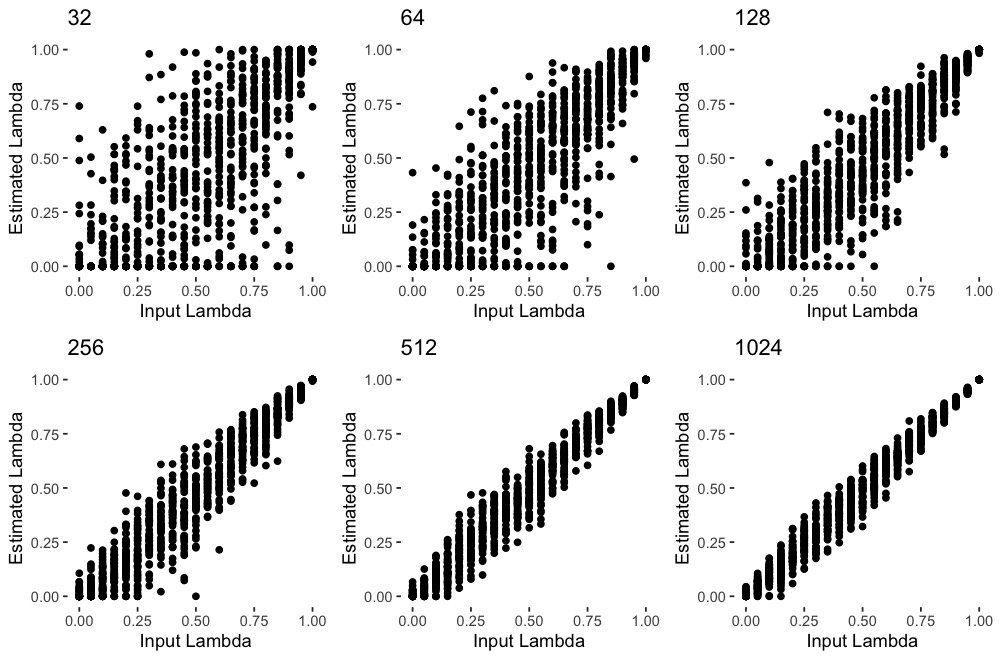
\includegraphics[width=0.95\linewidth]{Fig1}

\singlespacing \textbf{Figure 1}. Accuracy of Pagel's lambda estimations
across known lambda inputs on various tree sizes. As trees increase in
size, the estimates more closely resemble the input lambdas, however
considerable and concerning variation is apparent in trees smaller than
those with 200 tips. \hfill\break

\newpage

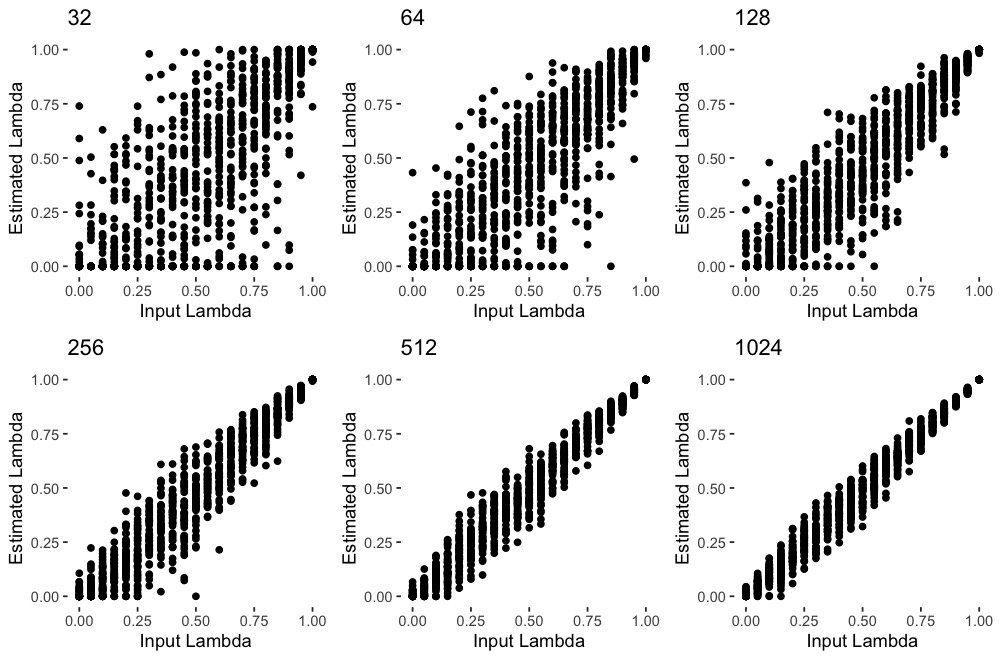
\includegraphics[width=0.95\linewidth]{Fig2}

\singlespacing \textbf{Figure 2}. Estimated ANOVA slopes under PGLS.
Across tree sizes, the mean estimated slope matches the input slope, and
as trees increase in size, the variance around this mean estimate
decreases. However, for trees with fewer than 200 tips, the error around
the estimated slope is considerable, where these analyses frequently
estimate slopes in the opposite direction of the known pattern.
\hfill\break

\newpage

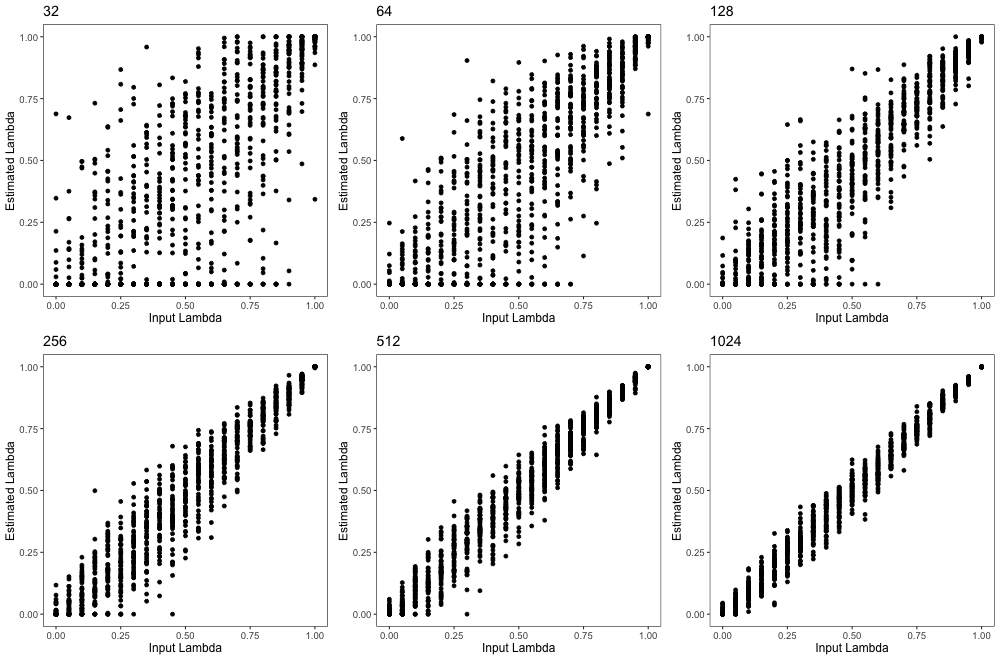
\includegraphics[width=0.95\linewidth]{Fig3}

\singlespacing \textbf{Figure 3}. Frequency of estimated lambda values
published in manuscripts in 2019. The majority of these values were
close to 0 or 1, and from phylogenies with fewer than 200 taxa.

\end{document}
